\chapter{Ανάλυση και Αρχική Σχεδίαση σε UML}
	
\section{Διαγράμματα Περιπτώσεων Χρήσης (use case diagrams)}

\begin{enumerate}
	\item FAQ: Ένας πελάτης βλέπει τα FAQ και ο υπάλληλος υποδοχής μπορεί να τα επεξεργαστεί  
	\item Chat:  Ένας πελάτης επικοινωνεί με τον υπάλληλος υποδοχής και αντίστροφα
	\item Καθαρισμός Δωματίων: Μία καμαριέρα αναφέρει τον αριθμό των αντικειμένων κάθε δωματίου
	\item Room service:  Ένας πελάτης ζητάει γεύμα στο δωμάτιο του και μία καμαριέρα απαντά στο αίτημα του
\end{enumerate}

\begin{figure}[H]
	\centering
	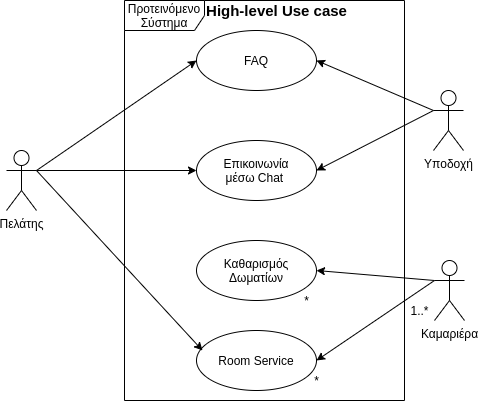
\includegraphics[width=0.8\textwidth]{Images/High_level_use_case}
	\caption{High Level Use Case Diagram}
	\label{high_level_use_case}
\end{figure}
\clearpage

\begin{enumerate}
	\item Επιλογή Γεύματος: Ο πελάτης επιλέγει μεταξύ πρωινού και βραδινού γεύματος
	\item Επιλογή Ώρας: Ο πελάτης επιλέγει την ώρα παράδοσης του γεύματος
	\item Αποστολή Παραγγελίας:  Ο πελάτης στέλνει την ολοκληρωμένη παραγγελία του και αναμένει απάντηση
	\item Ειδοποίηση Καμαριέρα: Το σύστημα στέλνει ειδοποίηση στην καμαριέρα αναγράφοντας τα αιτούμενα πιάτα
	\item Έλεγχος Προμηθειών: Η καμαριέρα ελέγχει εαν επαρκούν οι προμήθειες για την την παρασκευή του γεύματος
	\item Ειδοποίηση Πελάτη: Το σύστημα στέλνει ειδοποίηση στον πελάτη, ανάλογα με την απάντηση της καμαριέρας
\end{enumerate}

\begin{table}[H]
	\resizebox{\textwidth}{!}{%
		\begin{tabular}{|c|c|}
			\hline
			\textbf{Ενέργεια Συντελεστή} & \textbf{Γεγονός/Απόκριση Συστήματος}                                                  													  \\ \hline
			Επιλογή Γεύματος                       & \begin{tabular}[c]{@{}c@{}}Εμφάνιση επιλογών\\ Γευμάτων\end{tabular}                  				\\ \hline
			Επιλογή ώρας                 	      	   & Εμφάνιση επιλογών Ώρας                                                                																	   \\ \hline
			Αποστολή παραγγελίας           & \begin{tabular}[c]{@{}c@{}}Αποστολή ειδοποίησης στην\\ καμαριέρα\end{tabular}             \\ \hline
			Ειδοποίηση καμαριέρας          & Αποστολή ειδοποίησης στην καμαριέρα                                                     													\\ \hline
			Έλεγχος προμηθειών                & \begin{tabular}[c]{@{}c@{}}Φυσικός έλεγχος για την επάρκεια\\ των υλικών\end{tabular} \\ \hline
			Ειδοποίηση πελάτη                   & Αποστολή ειδοποίησης στον πελάτη                                                      													     \\ \hline
		\end{tabular}%
	}
\end{table}
\clearpage

\begin{figure}[H]
	\centering
	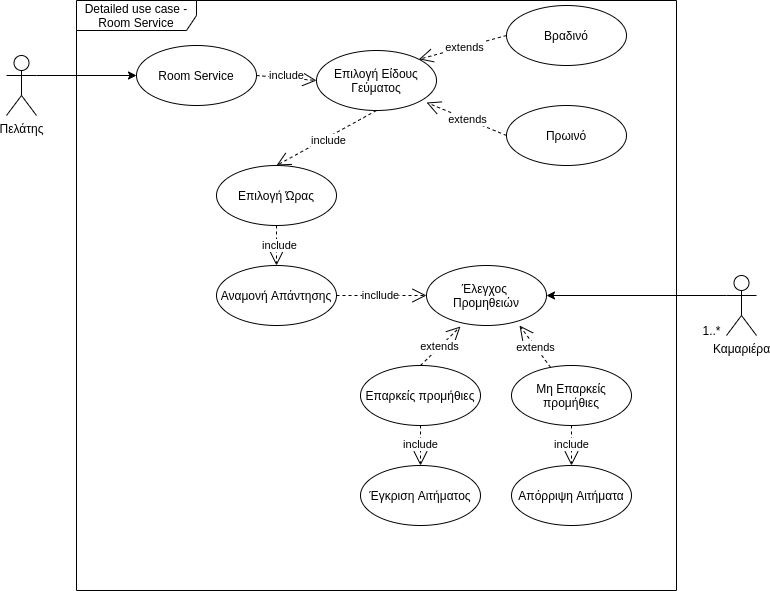
\includegraphics[width=1\textwidth]{Images/Low_level_use_case-Room service}
	\caption{High Level Use Case Diagram}
	\label{Low level use case - Room service}
\end{figure}

\section{Διαγράμματα Δραστηριοτήτων (Activity diagrams)}
\begin{figure}[H]
	\centering
	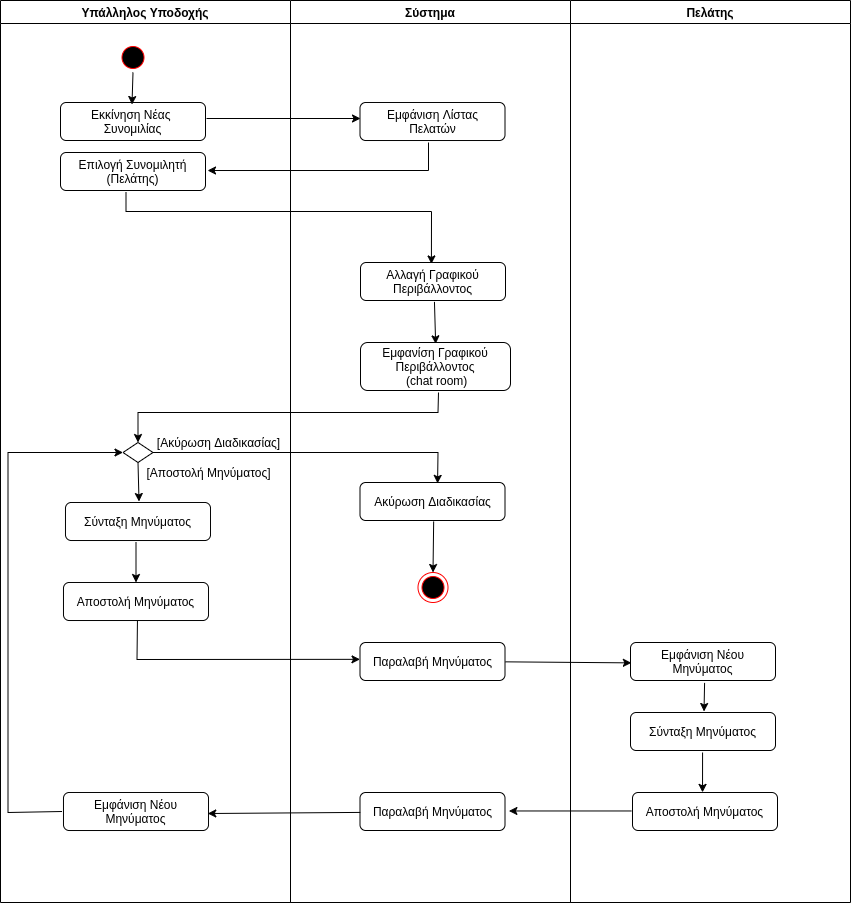
\includegraphics[width=0.9\textwidth]{Images/Activity-Chat}
	\caption{Activity Diagram - Επικοινωνία μέσω Chat}
	\label{Activity - Chat }
\end{figure}

\begin{figure}[H]
	\centering
	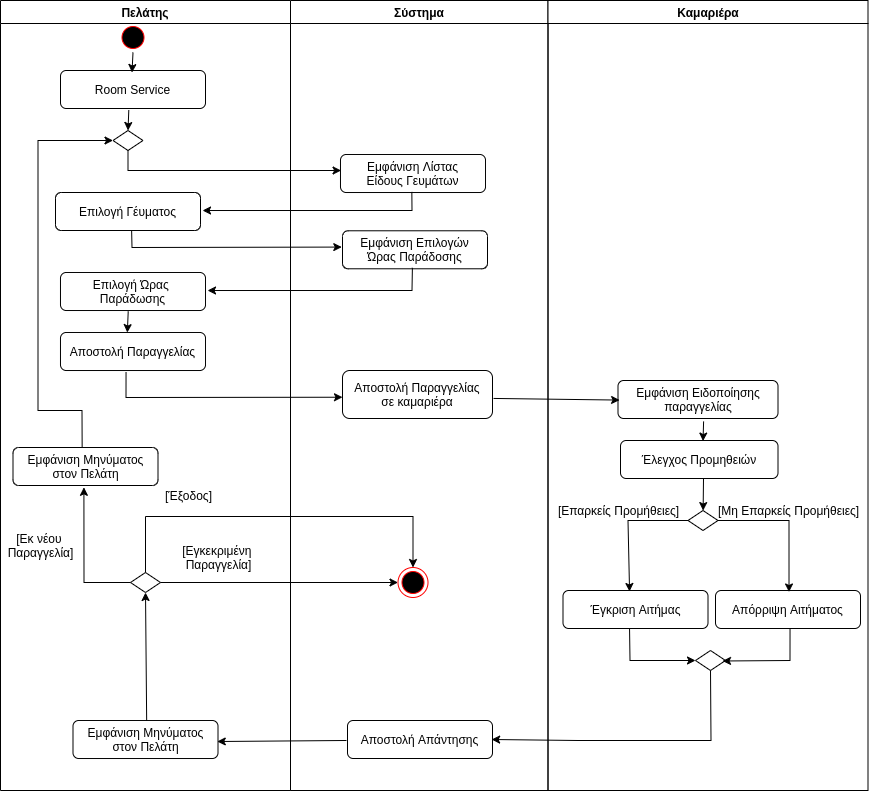
\includegraphics[width=1\textwidth]{Images/Activity-Room service}
		\caption{Activity Diagram - Room service}
		\label{Activity - Room service}
\end{figure}
\clearpage

\section{Ανάλυση και Επισκόπηση Σχεδίασης µε Διαγράμματα Κλάσεων (Class diagrams)}
\section{Διαγράμματα Ακολουθίας (sequence diagram) επιπέδου σχεδίασης}
\section{Μηχανές Καταστάσεων (state machines)}

